%!TEX root = ./main.tex



\tikzset{every picture/.style={line width=0.75pt}} %set default line width to 0.75pt        

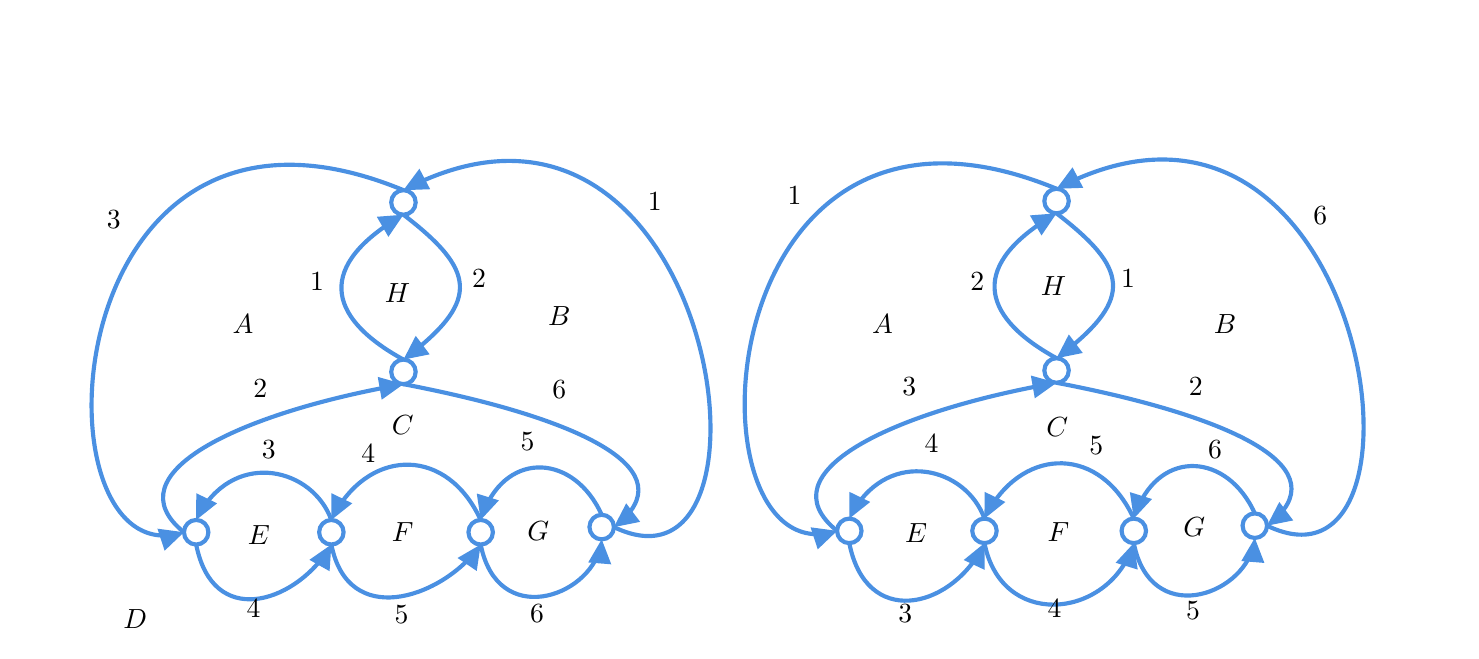
\begin{tikzpicture}[x=0.75pt,y=0.75pt,yscale=-1,xscale=1]
%uncomment if require: \path (0,877); %set diagram left start at 0, and has height of 877

%Shape: Ellipse [id:dp2062482206131232] 
\draw  [color={rgb, 255:red, 74; green, 144; blue, 226 }  ,draw opacity=1 ][line width=1.5]  (181.18,43.69) .. controls (181.18,40.42) and (183.82,37.77) .. (187.08,37.77) .. controls (190.33,37.77) and (192.97,40.42) .. (192.97,43.69) .. controls (192.97,46.95) and (190.33,49.6) .. (187.08,49.6) .. controls (183.82,49.6) and (181.18,46.95) .. (181.18,43.69) -- cycle ;
%Shape: Ellipse [id:dp42181631305663214] 
\draw  [color={rgb, 255:red, 74; green, 144; blue, 226 }  ,draw opacity=1 ][line width=1.5]  (181.18,125.31) .. controls (181.18,122.05) and (183.82,119.39) .. (187.08,119.39) .. controls (190.33,119.39) and (192.97,122.05) .. (192.97,125.31) .. controls (192.97,128.58) and (190.33,131.23) .. (187.08,131.23) .. controls (183.82,131.23) and (181.18,128.58) .. (181.18,125.31) -- cycle ;
%Shape: Ellipse [id:dp1893981875046039] 
\draw  [color={rgb, 255:red, 74; green, 144; blue, 226 }  ,draw opacity=1 ][line width=1.5]  (81.33,202.58) .. controls (81.33,199.31) and (83.97,196.66) .. (87.22,196.66) .. controls (90.48,196.66) and (93.11,199.31) .. (93.11,202.58) .. controls (93.11,205.85) and (90.48,208.5) .. (87.22,208.5) .. controls (83.97,208.5) and (81.33,205.85) .. (81.33,202.58) -- cycle ;
%Shape: Ellipse [id:dp3630097335542829] 
\draw  [color={rgb, 255:red, 74; green, 144; blue, 226 }  ,draw opacity=1 ][line width=1.5]  (276.69,200.09) .. controls (276.69,196.82) and (279.33,194.17) .. (282.59,194.17) .. controls (285.84,194.17) and (288.48,196.82) .. (288.48,200.09) .. controls (288.48,203.36) and (285.84,206.01) .. (282.59,206.01) .. controls (279.33,206.01) and (276.69,203.36) .. (276.69,200.09) -- cycle ;
%Shape: Ellipse [id:dp12213112120599945] 
\draw  [color={rgb, 255:red, 74; green, 144; blue, 226 }  ,draw opacity=1 ][line width=1.5]  (146.45,202.58) .. controls (146.45,199.31) and (149.09,196.66) .. (152.34,196.66) .. controls (155.6,196.66) and (158.24,199.31) .. (158.24,202.58) .. controls (158.24,205.85) and (155.6,208.5) .. (152.34,208.5) .. controls (149.09,208.5) and (146.45,205.85) .. (146.45,202.58) -- cycle ;
%Shape: Ellipse [id:dp14956651149377553] 
\draw  [color={rgb, 255:red, 74; green, 144; blue, 226 }  ,draw opacity=1 ][line width=1.5]  (218.4,202.58) .. controls (218.4,199.31) and (221.03,196.66) .. (224.29,196.66) .. controls (227.54,196.66) and (230.18,199.31) .. (230.18,202.58) .. controls (230.18,205.85) and (227.54,208.5) .. (224.29,208.5) .. controls (221.03,208.5) and (218.4,205.85) .. (218.4,202.58) -- cycle ;
%Curve Lines [id:da13558369698297235] 
\draw [color={rgb, 255:red, 74; green, 144; blue, 226 }  ,draw opacity=1 ][line width=1.5]    (190.32,116.91) .. controls (224.15,90.46) and (221.37,75.9) .. (187.08,49.6) ;
\draw [shift={(187.08,119.39)}, rotate = 323] [fill={rgb, 255:red, 74; green, 144; blue, 226 }  ,fill opacity=1 ][line width=0.08]  [draw opacity=0] (11.61,-5.58) -- (0,0) -- (11.61,5.58) -- cycle    ;
%Curve Lines [id:da08096805629350934] 
\draw [color={rgb, 255:red, 74; green, 144; blue, 226 }  ,draw opacity=1 ][line width=1.5]    (187.08,119.39) .. controls (153.21,100.86) and (142.93,76.71) .. (183.83,51.54) ;
\draw [shift={(187.08,49.6)}, rotate = 149.92] [fill={rgb, 255:red, 74; green, 144; blue, 226 }  ,fill opacity=1 ][line width=0.08]  [draw opacity=0] (11.61,-5.58) -- (0,0) -- (11.61,5.58) -- cycle    ;
%Curve Lines [id:da46118430818328493] 
\draw [color={rgb, 255:red, 74; green, 144; blue, 226 }  ,draw opacity=1 ][line width=1.5]    (81.33,202.58) .. controls (46.2,174.35) and (108.26,145.51) .. (183.62,131.85) ;
\draw [shift={(187.08,131.23)}, rotate = 170.12] [fill={rgb, 255:red, 74; green, 144; blue, 226 }  ,fill opacity=1 ][line width=0.08]  [draw opacity=0] (11.61,-5.58) -- (0,0) -- (11.61,5.58) -- cycle    ;
%Curve Lines [id:da12684350601217753] 
\draw [color={rgb, 255:red, 74; green, 144; blue, 226 }  ,draw opacity=1 ][line width=1.5]    (292.05,197.16) .. controls (321.77,170.32) and (267.27,146.57) .. (187.08,131.23) ;
\draw [shift={(288.48,200.09)}, rotate = 323] [fill={rgb, 255:red, 74; green, 144; blue, 226 }  ,fill opacity=1 ][line width=0.08]  [draw opacity=0] (11.61,-5.58) -- (0,0) -- (11.61,5.58) -- cycle    ;
%Curve Lines [id:da12533726813089074] 
\draw [color={rgb, 255:red, 74; green, 144; blue, 226 }  ,draw opacity=1 ][line width=1.5]    (288.48,200.09) .. controls (375.8,242.25) and (338.78,-38.85) .. (189.34,36.6) ;
\draw [shift={(187.08,37.77)}, rotate = 332.3] [fill={rgb, 255:red, 74; green, 144; blue, 226 }  ,fill opacity=1 ][line width=0.08]  [draw opacity=0] (11.61,-5.58) -- (0,0) -- (11.61,5.58) -- cycle    ;
%Curve Lines [id:da052098391594170956] 
\draw [color={rgb, 255:red, 74; green, 144; blue, 226 }  ,draw opacity=1 ][line width=1.5]    (76.95,203.7) .. controls (7.03,216.62) and (19.32,-31.54) .. (187.08,37.77) ;
\draw [shift={(81.33,202.58)}, rotate = 161.99] [fill={rgb, 255:red, 74; green, 144; blue, 226 }  ,fill opacity=1 ][line width=0.08]  [draw opacity=0] (11.61,-5.58) -- (0,0) -- (11.61,5.58) -- cycle    ;
%Curve Lines [id:da545296203025464] 
\draw [color={rgb, 255:red, 74; green, 144; blue, 226 }  ,draw opacity=1 ][line width=1.5]    (87.22,208.5) .. controls (95.26,249.18) and (133.74,236.79) .. (150.38,211.7) ;
\draw [shift={(152.34,208.5)}, rotate = 119.46] [fill={rgb, 255:red, 74; green, 144; blue, 226 }  ,fill opacity=1 ][line width=0.08]  [draw opacity=0] (11.61,-5.58) -- (0,0) -- (11.61,5.58) -- cycle    ;
%Curve Lines [id:da5810485905154714] 
\draw [color={rgb, 255:red, 74; green, 144; blue, 226 }  ,draw opacity=1 ][line width=1.5]    (152.34,208.5) .. controls (160.38,249.18) and (203.97,234.33) .. (222.15,211.41) ;
\draw [shift={(224.29,208.5)}, rotate = 124.16] [fill={rgb, 255:red, 74; green, 144; blue, 226 }  ,fill opacity=1 ][line width=0.08]  [draw opacity=0] (11.61,-5.58) -- (0,0) -- (11.61,5.58) -- cycle    ;
%Curve Lines [id:da14849415068653748] 
\draw [color={rgb, 255:red, 74; green, 144; blue, 226 }  ,draw opacity=1 ][line width=1.5]    (224.29,208.5) .. controls (232.28,248.97) and (276.2,234.31) .. (282.02,209.57) ;
\draw [shift={(282.59,206.01)}, rotate = 94.63] [fill={rgb, 255:red, 74; green, 144; blue, 226 }  ,fill opacity=1 ][line width=0.08]  [draw opacity=0] (11.61,-5.58) -- (0,0) -- (11.61,5.58) -- cycle    ;
%Curve Lines [id:da46264718836376073] 
\draw [color={rgb, 255:red, 74; green, 144; blue, 226 }  ,draw opacity=1 ][line width=1.5]    (89.34,192.72) .. controls (107.05,162.8) and (143.41,171.84) .. (152.34,196.66) ;
\draw [shift={(87.22,196.66)}, rotate = 295.84] [fill={rgb, 255:red, 74; green, 144; blue, 226 }  ,fill opacity=1 ][line width=0.08]  [draw opacity=0] (11.61,-5.58) -- (0,0) -- (11.61,5.58) -- cycle    ;
%Curve Lines [id:da44941926103098273] 
\draw [color={rgb, 255:red, 74; green, 144; blue, 226 }  ,draw opacity=1 ][line width=1.5]    (154.46,192.67) .. controls (172.13,161.99) and (208.21,161.67) .. (224.29,196.66) ;
\draw [shift={(152.34,196.66)}, rotate = 295.84] [fill={rgb, 255:red, 74; green, 144; blue, 226 }  ,fill opacity=1 ][line width=0.08]  [draw opacity=0] (11.61,-5.58) -- (0,0) -- (11.61,5.58) -- cycle    ;
%Curve Lines [id:da22225476038038006] 
\draw [color={rgb, 255:red, 74; green, 144; blue, 226 }  ,draw opacity=1 ][line width=1.5]    (225.66,192.76) .. controls (237.53,162.85) and (269.49,165.16) .. (282.59,194.17) ;
\draw [shift={(224.29,196.66)}, rotate = 287.25] [fill={rgb, 255:red, 74; green, 144; blue, 226 }  ,fill opacity=1 ][line width=0.08]  [draw opacity=0] (11.61,-5.58) -- (0,0) -- (11.61,5.58) -- cycle    ;
%Shape: Ellipse [id:dp42372727795787335] 
\draw  [color={rgb, 255:red, 74; green, 144; blue, 226 }  ,draw opacity=1 ][line width=1.5]  (495.85,43.02) .. controls (495.85,39.75) and (498.49,37.1) .. (501.74,37.1) .. controls (505,37.1) and (507.63,39.75) .. (507.63,43.02) .. controls (507.63,46.29) and (505,48.94) .. (501.74,48.94) .. controls (498.49,48.94) and (495.85,46.29) .. (495.85,43.02) -- cycle ;
%Shape: Ellipse [id:dp1870179348026778] 
\draw  [color={rgb, 255:red, 74; green, 144; blue, 226 }  ,draw opacity=1 ][line width=1.5]  (495.85,124.65) .. controls (495.85,121.38) and (498.49,118.73) .. (501.74,118.73) .. controls (505,118.73) and (507.63,121.38) .. (507.63,124.65) .. controls (507.63,127.92) and (505,130.57) .. (501.74,130.57) .. controls (498.49,130.57) and (495.85,127.92) .. (495.85,124.65) -- cycle ;
%Shape: Ellipse [id:dp6111256363608131] 
\draw  [color={rgb, 255:red, 74; green, 144; blue, 226 }  ,draw opacity=1 ][line width=1.5]  (396,201.92) .. controls (396,198.65) and (398.64,196) .. (401.89,196) .. controls (405.14,196) and (407.78,198.65) .. (407.78,201.92) .. controls (407.78,205.18) and (405.14,207.83) .. (401.89,207.83) .. controls (398.64,207.83) and (396,205.18) .. (396,201.92) -- cycle ;
%Shape: Ellipse [id:dp9315304169845421] 
\draw  [color={rgb, 255:red, 74; green, 144; blue, 226 }  ,draw opacity=1 ][line width=1.5]  (591.36,199.42) .. controls (591.36,196.15) and (594,193.5) .. (597.25,193.5) .. controls (600.51,193.5) and (603.15,196.15) .. (603.15,199.42) .. controls (603.15,202.69) and (600.51,205.34) .. (597.25,205.34) .. controls (594,205.34) and (591.36,202.69) .. (591.36,199.42) -- cycle ;
%Shape: Ellipse [id:dp322536109170936] 
\draw  [color={rgb, 255:red, 74; green, 144; blue, 226 }  ,draw opacity=1 ][line width=1.5]  (461.12,201.92) .. controls (461.12,198.65) and (463.76,196) .. (467.01,196) .. controls (470.27,196) and (472.9,198.65) .. (472.9,201.92) .. controls (472.9,205.18) and (470.27,207.83) .. (467.01,207.83) .. controls (463.76,207.83) and (461.12,205.18) .. (461.12,201.92) -- cycle ;
%Shape: Ellipse [id:dp9620679121888993] 
\draw  [color={rgb, 255:red, 74; green, 144; blue, 226 }  ,draw opacity=1 ][line width=1.5]  (533.06,201.92) .. controls (533.06,198.65) and (535.7,196) .. (538.95,196) .. controls (542.21,196) and (544.85,198.65) .. (544.85,201.92) .. controls (544.85,205.18) and (542.21,207.83) .. (538.95,207.83) .. controls (535.7,207.83) and (533.06,205.18) .. (533.06,201.92) -- cycle ;
%Curve Lines [id:da7735261830071775] 
\draw [color={rgb, 255:red, 74; green, 144; blue, 226 }  ,draw opacity=1 ][line width=1.5]    (504.99,116.24) .. controls (538.81,89.8) and (536.03,75.23) .. (501.74,48.94) ;
\draw [shift={(501.74,118.73)}, rotate = 323] [fill={rgb, 255:red, 74; green, 144; blue, 226 }  ,fill opacity=1 ][line width=0.08]  [draw opacity=0] (11.61,-5.58) -- (0,0) -- (11.61,5.58) -- cycle    ;
%Curve Lines [id:da5332538798838518] 
\draw [color={rgb, 255:red, 74; green, 144; blue, 226 }  ,draw opacity=1 ][line width=1.5]    (501.74,118.73) .. controls (467.88,100.2) and (457.6,76.04) .. (498.5,50.88) ;
\draw [shift={(501.74,48.94)}, rotate = 149.92] [fill={rgb, 255:red, 74; green, 144; blue, 226 }  ,fill opacity=1 ][line width=0.08]  [draw opacity=0] (11.61,-5.58) -- (0,0) -- (11.61,5.58) -- cycle    ;
%Curve Lines [id:da7801197789531258] 
\draw [color={rgb, 255:red, 74; green, 144; blue, 226 }  ,draw opacity=1 ][line width=1.5]    (396,201.92) .. controls (360.87,173.68) and (422.92,144.84) .. (498.29,131.18) ;
\draw [shift={(501.74,130.57)}, rotate = 170.12] [fill={rgb, 255:red, 74; green, 144; blue, 226 }  ,fill opacity=1 ][line width=0.08]  [draw opacity=0] (11.61,-5.58) -- (0,0) -- (11.61,5.58) -- cycle    ;
%Curve Lines [id:da022731159174359417] 
\draw [color={rgb, 255:red, 74; green, 144; blue, 226 }  ,draw opacity=1 ][line width=1.5]    (606.71,196.49) .. controls (636.44,169.65) and (581.94,145.9) .. (501.74,130.57) ;
\draw [shift={(603.15,199.42)}, rotate = 323] [fill={rgb, 255:red, 74; green, 144; blue, 226 }  ,fill opacity=1 ][line width=0.08]  [draw opacity=0] (11.61,-5.58) -- (0,0) -- (11.61,5.58) -- cycle    ;
%Curve Lines [id:da8965305497852382] 
\draw [color={rgb, 255:red, 74; green, 144; blue, 226 }  ,draw opacity=1 ][line width=1.5]    (603.15,199.42) .. controls (690.47,241.58) and (653.45,-39.52) .. (504,35.93) ;
\draw [shift={(501.74,37.1)}, rotate = 332.3] [fill={rgb, 255:red, 74; green, 144; blue, 226 }  ,fill opacity=1 ][line width=0.08]  [draw opacity=0] (11.61,-5.58) -- (0,0) -- (11.61,5.58) -- cycle    ;
%Curve Lines [id:da10010639301698165] 
\draw [color={rgb, 255:red, 74; green, 144; blue, 226 }  ,draw opacity=1 ][line width=1.5]    (391.62,203.04) .. controls (321.7,215.96) and (333.99,-32.21) .. (501.74,37.1) ;
\draw [shift={(396,201.92)}, rotate = 161.99] [fill={rgb, 255:red, 74; green, 144; blue, 226 }  ,fill opacity=1 ][line width=0.08]  [draw opacity=0] (11.61,-5.58) -- (0,0) -- (11.61,5.58) -- cycle    ;
%Curve Lines [id:da20611488989151905] 
\draw [color={rgb, 255:red, 74; green, 144; blue, 226 }  ,draw opacity=1 ][line width=1.5]    (401.89,207.83) .. controls (409.97,248.72) and (449.43,239.72) .. (465.37,211.03) ;
\draw [shift={(467.01,207.83)}, rotate = 115.22] [fill={rgb, 255:red, 74; green, 144; blue, 226 }  ,fill opacity=1 ][line width=0.08]  [draw opacity=0] (11.61,-5.58) -- (0,0) -- (11.61,5.58) -- cycle    ;
%Curve Lines [id:da6184979101341241] 
\draw [color={rgb, 255:red, 74; green, 144; blue, 226 }  ,draw opacity=1 ][line width=1.5]    (467.01,207.83) .. controls (475.09,248.72) and (524.06,244.69) .. (537.62,211.55) ;
\draw [shift={(538.95,207.83)}, rotate = 107.19] [fill={rgb, 255:red, 74; green, 144; blue, 226 }  ,fill opacity=1 ][line width=0.08]  [draw opacity=0] (11.61,-5.58) -- (0,0) -- (11.61,5.58) -- cycle    ;
%Curve Lines [id:da10958800394354862] 
\draw [color={rgb, 255:red, 74; green, 144; blue, 226 }  ,draw opacity=1 ][line width=1.5]    (538.95,207.83) .. controls (546.95,248.3) and (590.86,233.64) .. (596.69,208.9) ;
\draw [shift={(597.25,205.34)}, rotate = 94.63] [fill={rgb, 255:red, 74; green, 144; blue, 226 }  ,fill opacity=1 ][line width=0.08]  [draw opacity=0] (11.61,-5.58) -- (0,0) -- (11.61,5.58) -- cycle    ;
%Curve Lines [id:da7991255722818383] 
\draw [color={rgb, 255:red, 74; green, 144; blue, 226 }  ,draw opacity=1 ][line width=1.5]    (404,192.05) .. controls (421.71,162.14) and (458.08,171.17) .. (467.01,196) ;
\draw [shift={(401.89,196)}, rotate = 295.84] [fill={rgb, 255:red, 74; green, 144; blue, 226 }  ,fill opacity=1 ][line width=0.08]  [draw opacity=0] (11.61,-5.58) -- (0,0) -- (11.61,5.58) -- cycle    ;
%Curve Lines [id:da5824171246073673] 
\draw [color={rgb, 255:red, 74; green, 144; blue, 226 }  ,draw opacity=1 ][line width=1.5]    (469.12,192) .. controls (486.8,161.32) and (522.88,161) .. (538.95,196) ;
\draw [shift={(467.01,196)}, rotate = 295.84] [fill={rgb, 255:red, 74; green, 144; blue, 226 }  ,fill opacity=1 ][line width=0.08]  [draw opacity=0] (11.61,-5.58) -- (0,0) -- (11.61,5.58) -- cycle    ;
%Curve Lines [id:da15923659585236594] 
\draw [color={rgb, 255:red, 74; green, 144; blue, 226 }  ,draw opacity=1 ][line width=1.5]    (540.33,192.09) .. controls (552.19,162.18) and (584.15,164.49) .. (597.25,193.5) ;
\draw [shift={(538.95,196)}, rotate = 287.25] [fill={rgb, 255:red, 74; green, 144; blue, 226 }  ,fill opacity=1 ][line width=0.08]  [draw opacity=0] (11.61,-5.58) -- (0,0) -- (11.61,5.58) -- cycle    ;

% Text Node
\draw (103.33,96.4) node [anchor=north west][inner sep=0.75pt]    {$A$};
% Text Node
\draw (255.33,92.4) node [anchor=north west][inner sep=0.75pt]    {$B$};
% Text Node
\draw (180,145.07) node [anchor=north west][inner sep=0.75pt]    {$C$};
% Text Node
\draw (50.67,238.4) node [anchor=north west][inner sep=0.75pt]    {$D$};
% Text Node
\draw (110.67,197.73) node [anchor=north west][inner sep=0.75pt]    {$E$};
% Text Node
\draw (180,196.4) node [anchor=north west][inner sep=0.75pt]    {$F$};
% Text Node
\draw (245.33,196.07) node [anchor=north west][inner sep=0.75pt]    {$G$};
% Text Node
\draw (176.67,81.4) node [anchor=north west][inner sep=0.75pt]    {$H$};
% Text Node
\draw (411.33,96.07) node [anchor=north west][inner sep=0.75pt]    {$A$};
% Text Node
\draw (576,96.4) node [anchor=north west][inner sep=0.75pt]    {$B$};
% Text Node
\draw (492.67,78.07) node [anchor=north west][inner sep=0.75pt]    {$H$};
% Text Node
\draw (495.33,145.73) node [anchor=north west][inner sep=0.75pt]    {$C$};
% Text Node
\draw (427.33,197.07) node [anchor=north west][inner sep=0.75pt]    {$E$};
% Text Node
\draw (496,196.4) node [anchor=north west][inner sep=0.75pt]    {$F$};
% Text Node
\draw (561.33,194.07) node [anchor=north west][inner sep=0.75pt]    {$G$};
% Text Node
\draw (140.67,76.07) node [anchor=north west][inner sep=0.75pt]    {$1$};
% Text Node
\draw (303.33,37.4) node [anchor=north west][inner sep=0.75pt]    {$1$};
% Text Node
\draw (218.67,74.4) node [anchor=north west][inner sep=0.75pt]    {$2$};
% Text Node
\draw (113.33,127.73) node [anchor=north west][inner sep=0.75pt]    {$2$};
% Text Node
\draw (257.33,128.07) node [anchor=north west][inner sep=0.75pt]    {$6$};
% Text Node
\draw (246.67,236.07) node [anchor=north west][inner sep=0.75pt]    {$6$};
% Text Node
\draw (181.33,236.4) node [anchor=north west][inner sep=0.75pt]    {$5$};
% Text Node
\draw (242,153.07) node [anchor=north west][inner sep=0.75pt]    {$5$};
% Text Node
\draw (165.33,158.73) node [anchor=north west][inner sep=0.75pt]    {$4$};
% Text Node
\draw (110,233.4) node [anchor=north west][inner sep=0.75pt]    {$4$};
% Text Node
\draw (117.33,156.73) node [anchor=north west][inner sep=0.75pt]    {$3$};
% Text Node
\draw (42.67,46.07) node [anchor=north west][inner sep=0.75pt]    {$3$};
% Text Node
\draw (573.33,156.73) node [anchor=north west][inner sep=0.75pt]    {$6$};
% Text Node
\draw (516,155.07) node [anchor=north west][inner sep=0.75pt]    {$5$};
% Text Node
\draw (436.67,154.07) node [anchor=north west][inner sep=0.75pt]    {$4$};
% Text Node
\draw (424,236.07) node [anchor=north west][inner sep=0.75pt]    {$3$};
% Text Node
\draw (496,233.73) node [anchor=north west][inner sep=0.75pt]    {$4$};
% Text Node
\draw (562.67,234.4) node [anchor=north west][inner sep=0.75pt]    {$5$};
% Text Node
\draw (426,126.73) node [anchor=north west][inner sep=0.75pt]    {$3$};
% Text Node
\draw (564,126.4) node [anchor=north west][inner sep=0.75pt]    {$2$};
% Text Node
\draw (458.67,76.07) node [anchor=north west][inner sep=0.75pt]    {$2$};
% Text Node
\draw (531.33,74.73) node [anchor=north west][inner sep=0.75pt]    {$1$};
% Text Node
\draw (370.67,34.4) node [anchor=north west][inner sep=0.75pt]    {$1$};
% Text Node
\draw (624,44.07) node [anchor=north west][inner sep=0.75pt]    {$6$};


\end{tikzpicture}